\section{MaxPartitions algorithm}%
\label{sec:maxParts}

Since state space discretization for Reinforcement Learning is usually done
\textit{before} any learning takes place, the discretization is likely to create
adjacent discrete states that are mapped to the same optimal action. The
question we would then like to answer is this: if $\mathcal{T}$ is a decision
tree representing a trained strategy and $\mathcal{A}_{\mathcal{T}}$ is its
induced partitioning, can we find another partitioning $\mathcal{B}$ which is
smaller than $\mathcal{A}_{\mathcal{T}}$ but still respects $\mathcal{T}$?

As an example, we can consider the toy strategy from
Example~\ref{ex:runningExample}. In Figure~\ref{fig:complexExample} the strategy
is represented as a decision tree (\ref{fig:complexExampleTree}) by omitting the
specification of cost values of each action and only preserving the optimal
action for each discrete state. On the right (\ref{fig:complexExample2dVisual})
is a 2D visualization of the induced partitioning of the state space. It can
easily be assessed, that the partitioning has several redundant splits where
areas of the same color (meaning they suggests the same optimal action) are
split in two. For instance, the region $((0,0),(1,1))$ and the region
$((0,1),(1,2))$ both specify $a$ as the optimal action, and we could replace
these two regions with a single one given by $((0,0),(1,2))$.  Since each region
is represented in our decision tree as a leaf node, the fewer regions we have
the smaller a tree we need to represent it.

\begin{figure}[ht]
    \begin{subfigure}[b]{.5\textwidth}
        \centering
        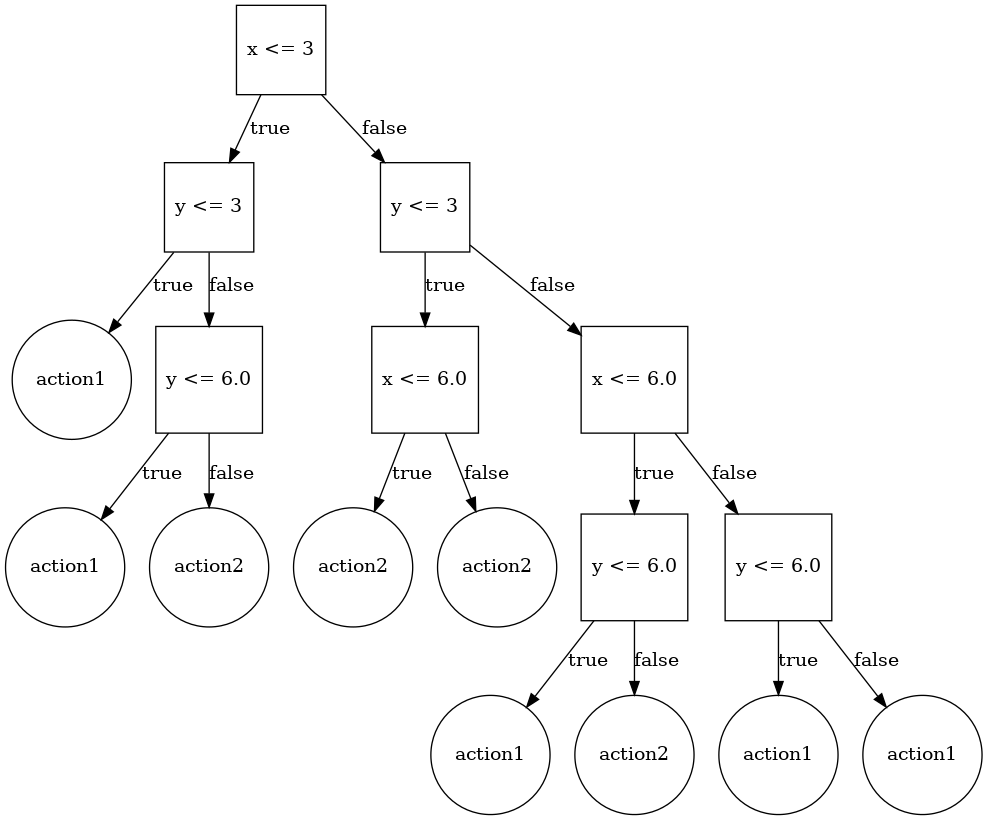
\includegraphics[width=\textwidth]{complexExampleTree}
        \subcaption{%
            % Tree representation of strategy with 2 state dimensions and 3
            % actions
        }\label{fig:complexExampleTree}
    \end{subfigure}
    \begin{subfigure}[b]{.5\textwidth}
        \centering
        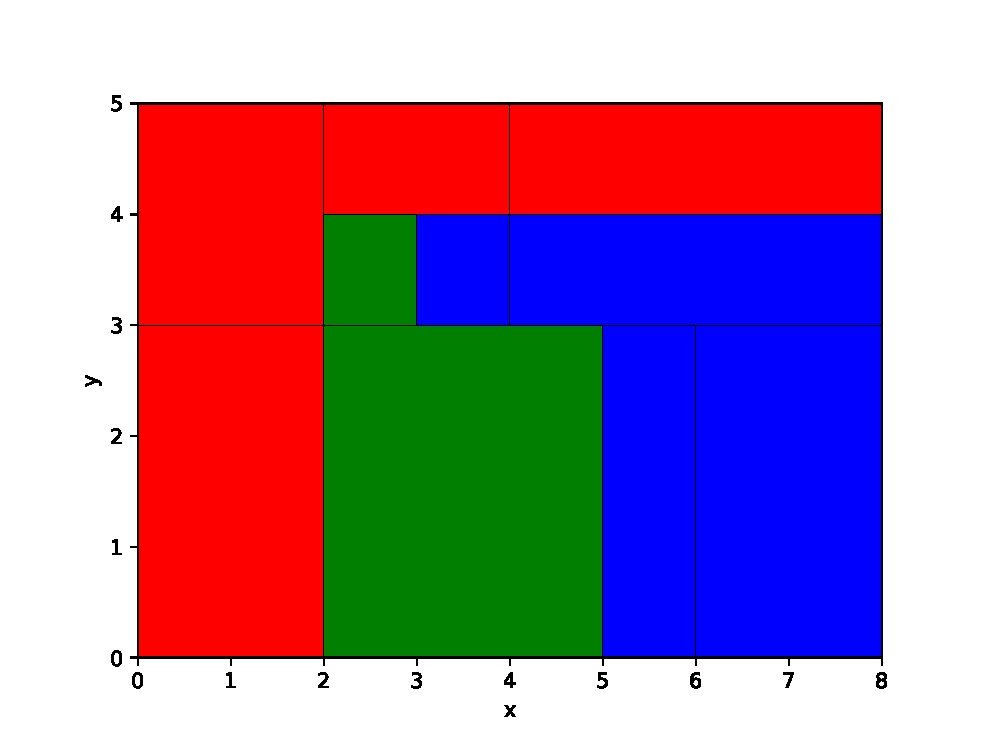
\includegraphics[width=\textwidth]{complexExample2dVisual}
        \subcaption{%
            % 2D visualization of the state space partitioning entailed by the
            % decision tree.
        }\label{fig:complexExample2dVisual}
    \end{subfigure}%

    \caption{%
        Two representations of the toy strategy introduced in
        Example~\ref{ex:runningExample}. In~\subref{fig:complexExampleTree} the
        Q-table is represented as a decision tree.
        In~\subref{fig:complexExample2dVisual} a 2D visualization of the state
        space partitioning is showed, where the colors indicate what the optimal
        action is in that area of the state space (red for $a$, green for $b$
        and blue for $c$).
    }%
    \label{fig:complexExample}
\end{figure}

We start by stating the problem of finding maximum sized regions as a problem of
local optimization: Given a starting point $s^{\min}$, find $s^{\max}$ such that
$\nu = (s^{\min}, s^{\max})$ has singular mapping in $\mathcal{T}$ while no
other region $\nu' = (s^{\min}, s')$ where $s'_j = s^{\max}_j$ for $j =
1,\ldots,i-1,i+1,\ldots,K$ and $s'_i > s^{\max}_i$ has this property.


\subsection{Details of the algorithm}%
\label{sub:maxPartsDescription}

We introduce a new notation to refer to individual bounds on the dimensions in
$\mathcal{T}$. We denote by $\mathcal{T}_i$ the sorted list of bounds on
dimension $i$ and by $\mathcal{T}_{i,j}$ the $j$th smallest bound on dimension
$i$ for each $j = 1,2,\ldots,|\mathcal{T}_i|$. This can be precomputed as a
matrix in log-linear time by collecting and sorting the bounds on all branch
nodes in $\mathcal{T}$ and allows accessing $\mathcal{T}_{i,j}$ in constant
time.

Exploiting this notation, if $p$ is a $K$-dimensional vector of index pointers
to bounds in $\mathcal{T}$, such that $p_i \in p$ is a pointer to
$\mathcal{T}_{i,p_i}$, then we can define a point at an intersection of bounds
in all $K$ dimensions as $s^{p}_{\mathcal{T}} =
(\mathcal{T}_{1,p_1},\mathcal{T}_{2,p_2},\ldots,\mathcal{T}_{K,p_K})$. We will
omit the subscript $\mathcal{T}$ on $s^{p}_{\mathcal{T}}$ when it is clear from
the context.

For the algorithm, we require that the domain of $\mathcal{T}$ is bounded in all
$K$ dimensions. This can be achieved by including a minimum and a maximum bound
for each dimension $i$, which is not represented by a branch node in
$\mathcal{T}$. These limit bounds can be negative and positive infinity, in
which case we say $\mathcal{T}_{i,1} = -\infty$ and
$\mathcal{T}_{i,|\mathcal{T}_{i}|} = \infty$. Further, in a slight abuse of
notation, we define $\mathcal{T}_{i,|\mathcal{T}_i| + 1}$ to be some
\textit{sentinel} value representing that we are outside the boundaries of
dimension $i$.  Correspondingly, we define a sentinel action $\alpha$, and we
say that $\mathcal{T}(s^p_{\mathcal{T}}) = \alpha$ if and only if $\exists p_i
\in p, p_i = |\mathcal{T}_i| + 1$.

The algorithm works by maintaining two vectors of index pointers, $p^{\min}$ and
$p^{\max}$, and iteratively increasing $p^{\max}$ until a region $\nu =
(s^{p^{\min}}, s^{p^{\max}})$ cannot be expanded further. The regions are stored
in a list $\mathcal{R}$ and a list $\mathcal{P}$ is keeping track of the
$p^{\min}$ vectors to use as starting points for the region search. Initially,
$\mathcal{R}$ is empty and $\mathcal{P}$ contains just a vector of $K$ ones
(ie.\ the vector pointing to the lowest bounds of all $K$ dimensions). The
algorithm is given in pseudo-code in Algorithm~\ref{alg:MaxPartitions} while the
following describes it in more detail.

Let $p^{\min}$ be the result of popping the lexicographically smallest element
of $\mathcal{P}$. We can then define $s^{\min} = s^{p^{\min}}$ as the `lower
left' corner in a region $\nu = (s^{\min}, s^{\max})$ where $s^{\max}$ is the
point we want to determine, so that $\nu$ has singular mapping in $\mathcal{T}$.
By definition, $s^{\max} = s^{p^{\max}}$ satifies this requirement for $p^{\max}
= (p^{\min}_{1} + 1, \ldots, p^{\max}_{K} + 1)$, since no branch node in
$\mathcal{T}$ splits on a predicate $c$ where $\mathcal{T}_{i,p^{\min}_{i}} < c
< \mathcal{T}_{i,p^{\min} + 1}$ for any $i = 1, \ldots, K$. 

We can now increase $p^{\max}$ by 1 in any dimension $i$ and test for singular
mapping in our new region. Additionally, we require that the point
$s^{p^{\max}}$ is not already covered by a region in $\mathcal{R}$, as this
would result in overlapping regions. Let $\mathbf{\hat{e}}_i$ denote the unit
vector parallel to axis $i$, such that $p + \mathbf{\hat{e}}_i = (p_1,\ldots,p_i
+ 1,\ldots,p_K)$. Then, the updated region is given by $\nu = (s^{\min},
s^{p^{\max} + \mathbf{\hat{e}}_{i}})$. If $|\mathcal{T}(\nu)| = 1$ and $\forall
\nu' \in \mathcal{R}, s^{p^{\max} + \mathbf{\hat{e}}_{i}} \notin \nu'$, then the
update did not violate the singular mapping property and we can set $p^{\max} =
p^{\max} + \mathbf{\hat{e}}_{i}$. Otherwise, we mark dimension $i$ as
\textit{exhausted} so we know not to increase in this dimension again. We then
continue, choosing a new dimension not marked as exhausted.

This process is repeated until all dimensions have been exhausted at which
point, $p^{\max}$ together with the unchanged $p^{\min}$ defines a region $\nu =
(s^{p^{\min}}, s^{p^{\max}})$ that has singular mapping in $\mathcal{T}$ and
cannot be expanded further in any dimension. More generally, we can say that
given $p^{\min}$ we want to choose $p^{\Delta} \in \mathbb{Z}^{K}$ such that
$\nu = (s^{p^{\min}}, s^{p^{\min} + p^{\Delta}})$ has singular mapping in
$\mathcal{T} $and no other $p^{\Delta'} > p^{\Delta}$ has this property.

Having found $\nu$, we add it to $\mathcal{R}$. Further, we add to $\mathcal{P}$
all the points we can create from taking $p^{\min}$ and setting $p^{\min}_{i} =
p^{\max}_{i}$ for all $i$ where $p^{\max}_{i} < |\mathcal{T}_{i}|$. These points
will later be popped and used as a new $p^{\min}$ for a search for a large
region. If $\mathcal{P}$ is not empty, we repeat the entire process, otherwise
the algorithm terminates and returns $\mathcal{R}$ which now represents a new
partitioning that respects $\mathcal{T}$.


% We can then define
% the following recursive function \textit{grow}, which, given a vector $p$ of
% index pointers to bounds in $\mathcal{T}$ and an initially empty set $E$, finds
% $p^{\max}$ such that the region $\nu = (s^{p^{\min}}, s^{p^{\max}})$ has
% singular mapping in $\mathcal{T}$ but cannot be expanded in any dimension
% without loosing this property:

% Let $M = \argmax_{i} |\mathcal{T}_i|$.

% \[
%     % grow_{\mathcal{T}}(p) = p + \Delta
%     grow_{\theta}(p, E) =
%     \begin{cases}
%         p & \text{if } |E|  =  K \\
%         grow(p, E \cup \{i\}) &
%             \text{if }
%                 |\mathcal{T}((s^{p^{\min}}, s^{p + \mathbf{\hat{e}}_i}))| > 1
%                 \text{~or $s^{p + \mathbf{\hat{e}}_i}$ is explored} \\
%         grow(p + \mathbf{\hat{e}}_i, E) & \text{otherwise}
%     \end{cases}
% \] 

% \noindent where $\Delta \in \{ 0,\ldots,M \}^K$ such that
% $|\mathcal{T}((s^{p}_{\mathcal{T}}, s^{p + \Delta}_{\mathcal{T}}))| = 1$ and for
% all $\nu \in \mathcal{R}, \nu \cap (s^{p}_{\mathcal{T}}, s^{p +
% \Delta^K}_{\mathcal{T}}) = \emptyset$ and where no other $\Delta'$
% lexicographically larger than $\Delta$ has this property.

% \noindent
% where $grow$ is parametized by $\theta = (\mathcal{T}, p^{\min})$ with
% $\mathcal{T}$ being a binary decision tree over the domain $\mathbb{R}^K$
% inducing a partitioning $\mathcal{A}_{\mathcal{T}}$ and $p^{\min}$ is
% a vector of index pointers giving the left lowest point of the region we are
% currently expanding. Further, to avoid cluttering the expression for $grow$,
% we use $i$ defined as

% \begin{align*}
%     i &= \argmin_{i \in \{ i \mid i = 1,\ldots,K, i \notin E, p_i \le 
%     |\mathcal{T}_i| \}}
%         \mathcal{T}_{i,p_i+1} - \mathcal{T}_{i,p_i} \\
% \end{align*}

% The \textsc{MaxPartitions} algorithm is given as pseudo-code in
% Algorithm~\ref{alg:MaxPartitions}.

\begin{algorithm}[!ht]
    \caption{MaxPartitions}\label{alg:MaxPartitions}

    \begin{algorithmic}[1]
        \Require{%
            $\mathcal{T}$: A binary decision tree over the domain
            $\mathbb{R}^K$ inducing the partitioning $\mathcal{A}_{\mathcal{T}}$
        }
        \State{$\mathcal{R} \gets \{\}$}
        \State{$\mathcal{P} \gets \{ \mathbf{1}^K \} $}\Comment{%
            $\mathbf{1}^K$ is a $K$-dimensional vector of ones
        }

        \While{$\mathcal{P}$ is not empty}
            \State{$p^{\min} \gets \min \mathcal{P}$}\Comment{Lexicographic min}
            \State{$\mathcal{P} \gets \mathcal{P} \setminus \{p^{\min}$\}}%
            \Comment{Remove $p^{\min}$ from $\mathcal{P}$}

            \If{$s^{p^{\min}}_{\mathcal{T}} \notin \mathcal{R}$}\Comment{%
                Check $s^{p^{\min}}_{\mathcal{T}}$ has not been covered yet
            }

                \State{%
                    $p^{\max} \gets p^{\min} + p^{\Delta}$
                    % $p^{\max} \gets grow(p^{\min})$
                    % $p^{\max} \gets grow(
                    %     p^{\min} + \mathbf{1}^K,
                    %     \emptyset \mid (\mathcal{T}, p^{\min})
                    % )$
                }\Comment{%
                    Select largest $p^{\Delta}$
                }

                \State{%
                    $\mathcal{R} \gets \mathcal{R} \cup \{
                        (s^{p^{\min}}_{\mathcal{T}},s^{p^{\max}}_{\mathcal{T}})
                    \}
                $}\Comment{%
                    Add new region to $\mathcal{R}$
                }

                \For{$i = 1, 2, \ldots, K$}\Comment{%
                    Add points to $\mathcal{P}$
                }
                    \If{%
                        $p^{\min}_i \neq p^{\max}_i$
                        \textbf{and} $p^{\max}_i < |\mathcal{T}_i|$
                    }
                        \State{$\mathcal{P} \gets \mathcal{P} \cup
                        \{(p^{\min}_1, \ldots, p^{\max}_i, \ldots,
                        p^{\min}_k)\}
                    $}
                    \EndIf%
                \EndFor%
            \EndIf%


        \EndWhile%

        \State{\textbf{return} $\mathcal{R}$}

    \end{algorithmic}

\end{algorithm}


\subsection{Analyzing the algorithm}%
\label{sub:maxPartsAnalysis}

In the following we provide an upper bound of the running time of
\textsc{MaxPartitions} and a proof of correctness.

\subsubsection{Running time}%
\label{sec:runningTime}

The first thing to notice is the outer while loop over $\mathcal{P}$. Points are
dynamically added to $\mathcal{P}$ every time a new region is constructed, and
in the worst case, $K$ new points (one for each dimension) are added for each
region. The number of regions that can be found and constructed is bounded by
the size of the original parition $\mathcal{A}_{\mathcal{T}}$, as the worst case
is when $\mathcal{A}_{\mathcal{T}}$ is already a minimal partitioning that
respects $\mathcal{T}$. In this case, the algorithm will produce $\mathcal{R} =
\mathcal{A}_{\mathcal{T}}$ and the number of regions will necessarily be the
same. Let $N = |\mathcal{A}_{\mathcal{T}}|$. Then we can state that the outer
while loop is bounded by $O(KN)$.

% Inside the loop, we first have an operation that pops the (lexicographically)
% smallest item of $\mathcal{P}$. This can be done in logarithmic time using an
% appropriate data structure (a priority queue) for $\mathcal{P}$. Of greater
% interest is the check for membership of a point $s$ in $\mathcal{R}$ (which is
% both checked for $s^{p^{\min}}$ and for each candidate of $p^{\max}$ in
% $s^{p^{\max}}$ in the search for $p^{\Delta}$). 

How about finding $p^{\Delta}$? The procedure is to increment by 1 in any one
unexhausted dimension and then check for the validity of that increment. This
check has two components: (a) check if the new region still has singular mapping
in $\mathcal{T}$ and (b) check if the new region overlaps with any region
already in $\mathcal{R}$. Let $\nu = (s^{\min}, s^{\max})$ be the candidate
region for some $p^{\Delta} = \mathbf{1}^{K} + \mathbf{\hat{e}}_{i}$ (ie.\ so
$s^{\max} = s^{p^{\min} + p^{\Delta}}$).

For (a), we have to query $\mathcal{T}(\nu)$ which visits all leaves in $l \in
\mathcal{T}$ for which $\lambda(l) \cap \nu \neq \emptyset$. Let us denote this
set by $\mathbf{L}_{\nu}$ and say has size $L$. The analysis of this operation
is complicated. First of all, we have no guarantee that the tree is balanced.
If we assume that it is, then the path from the root to a leaf is $O(\log T)$
where $T = (2N) - 1$ is the size of the tree.

Assuming the tree is balanced,
the length of the path from the root node to a leaf node is logarithmic in the
number size of the tree. However, to query $\mathcal{T}(\nu)$ we do not need to do a
$O(L \log N)$ operation. Consider two leaves, $l_{j}, l_{k} \in
\mathbf{L}_{\nu}$, that share the same path until their common parent node
splits them. We only need to follow the path to the parent once and then go to
$l_{j}$ and $l_{k}$ respectively. In general, if we by $\omega(l)$ denote the
set of nodes on the path from the root node to a leaf $l$, then we need
$|\bigcup_{l \in \mathbf{L}_{\nu}} \omega(l)|$ operations to retrieve
$\mathbf{L}_{\nu}$.


% For the running time, we first turn our attention to the outer while loop
% iterating through $\mathcal{P}$. Since $\mathcal{P}$ is dynamically grown, we
% must consider what the accumulated size during the entire run of the algorithm
% can amount to. For this, we look at the case where new points are added to
% $\mathcal{P}$, namely in line 27-31 where we have found a new region. We add a
% point for each of the $K$ variables, barring some edge cases. This means, that
% an upper bound to the number of points we must process in total is $K$ times the
% number of regions we find.

% The worst case number of regions the algorithm can find is on the other hand
% bounded by the number of partitions (or leaf nodes) in the original tree
% $\mathcal{T}$. This because either the partitioning $\mathcal{A}$ entailed by
% $\mathcal{T}$ is already optimal, in which case, the algorithm will just find
% one region for every leaf node in $\mathcal{T}$, or $\mathcal{A}$ is not
% optimal, meaning the algorithm will find fewer (but larger) regions. Therefore,
% the outer while loop is bounded by $O(KN)$ with $N$ being the number of leaf
% nodes in $\mathcal{T}$.

% Inside the while loop, we have two sorting operations and a for-loop. In line 6,
% we sort $\mathcal{P}$, but we ignore this in our analysis, as $\mathcal{P}$ is
% expected to at any time only contain a small subset of all the points entering
% and exiting $\mathcal{P}$ during the algorithm. Secondly, a smart data structure
% (eg.\ a heap) could sort the points at insertion and thus remove the need to
% sort every time.

% In line 11, however, we sort $\mathcal{C}$ according to the current $p^{\min}$.
% As presented here, this sorting is unavoidable as we cannot expect to know the
% correct sorting with respect to $p^{\min}$.\footnote{%
%     One could imagine, that $K$ lists with the bounds in $\mathcal{C}$ sorted
%     according their respective $V_i$ were stored and consulted in the following
%     for-loop, thus alleviating the need to sort $\mathcal{C}$ in every
%     iteration. This approach is not pursued here.
% } If we assume that the sorting operation is $O(C\log C)$ with $C$ being the
% size of $\mathcal{C}$, then question becomes one of estimating $C$. Also here we
% have that $C$ is proportional to $N$ and $K$, as $\mathcal{C}$ is constructed
% from all the predicates of the branch nodes in $\mathcal{T}$. This is at most
% $N$, or rather $N-1$. Something something $\approx O(KN^2\log N)$.

\subsection{From regions to decision tree}%
\label{sub:regionsToDT}

The output of the \textsc{MaxPartitions} algorithm is a list of regions with
associated actions. For this to be of any use, we need to construct a new
decision tree to represent these state-action pairs. To this goal, we face the
issue that it is not given (and in fact, very unlikely) that the suggested
partitioning can be perfectly represented by a decision tree, as this would
require the existence of enough `clean splits' (ie.\ predicates on some variable
that perfectly divides the regions into two sets with an empty disjunction) to
arrange the entire set of regions.

Therefore, we suggest a brute-force algorithm that tries to separate the regions
as cleanly as possible. Let $\mathbf{R}$ be a list of regions $\nu \in
\mathbf{R}$ with $a_{\nu}$ being the action associated with $\nu$. We
iteratively create a branch node that splits $\mathbf{R}$ into two,
$\mathbf{R}_{low}$ and $\mathbf{R}_{high}$, based on a predicate function
$\rho(x_i,c) = x_i \le c$ with $c \in \mathbb{R}$ so that $\mathbf{R}_{low} = \{
\nu \in \mathbf{R} \mid \nu_{i,\min} \le c \}$ and $\mathbf{R_{high}} = \{ \nu
\in \mathbf{R} \mid \nu_{i,\max} > c \}$. When the list only contains a single
element $\nu$, we create a leaf node with action $a_{\nu}$ and return.

The question is how to determine $\rho(x_i,c)$, more specifically which variable
$x_i$ to predicate on and at which value $c$. Ideally, we want to split
$\mathbf{R}$ in two equally sized subsets and in a way that no single region
would have to occur in both, ie.\ we would like $\mathbf{R}_{low} \cap
\mathbf{R}_{high} = \emptyset$. For this we define an impurity measure
$I(\mathbf{R}_{low},\mathbf{R}_{high})$ that penalises the difference in size
between $\mathbf{R}_{low}$ and $\mathbf{R}_{high}$ and the size of the
disjunction between the two. Let $abs(a)$ be the absolute value of $a$ and let
$|b|$ denote the size of a set $b$, then

\[
    I(\mathbf{R}_{low}, \mathbf{R}_{high})  = abs(|\mathbf{R}_{low}| -
    |\mathbf{R}_{high}|) + |\mathbf{R}_{low} \cap \mathbf{R}_{high}|
\]


Our brute-force way of finding the predicate that minimizes $I$ is to iterate
over the dimensions in $\mathcal{S}$ and for each dimension $i$ we sort the
regions according to their upper bound. Let $\mathbf{R}_i = \{ \nu^1, \nu^2,
\ldots, \nu^n \}$ be the list sorted according to the $i$ th dimension so that
for all $\nu^j, \nu^{j+1}$ it holds that $\nu^{j}_{i,\max} \le
\nu^{j+1}_{i,\max}$. If we then let $\rho(x_i,c) = x_i \le c$ with $c =
\nu^{j}_{i,\max}$ we have $|\mathbf{R}_{low}| = j$ and |$\mathbf{R}_{high}| = n
- j$. For determining the size of $\mathbf{R}_{low} \cap \mathbf{R}_{high}$ we
simply need to count the number of regions $\nu^{j+m}$ for $m = 1, 2, \ldots,
n-j$ whose lower bound is less than our predicate bound $c$, since these regions
will appear both in $\mathbf{R}_{low}$ (because then, by definition, $\rho(x_i,c) = x_i
\le c$ will be true for $x_i = \nu^{j+m}_{i,\min}$ and $c = \nu^{j}_{i,\max}$)
and in $\mathbf{R}_{high}$ (because our sorting ensures that for all
$\nu^{j},\nu^{j+m}$ it holds that $\nu^{j}_{i,\max} \le \nu^{j+m}_{i,\max}$).

Now we can write our impurity measure in terms of these quantities:

\[
    I(\mathbf{R}_{low}, \mathbf{R}_{high}) = abs(j - (n - j)) +
    \sum^{n}_{m=1} \mathbbm{1}(\rho(\nu^{j+m}_{i,\min},\nu^{j}_{i,\max})), \quad
    \text{for all }\nu^{j} \in \mathbf{R}
\] 

where $\mathbbm{1}$ is the indicator function, $\mathbf{R}$ is the list of
regions sorted according to upper bound and $\mathbf{R}_{low}$ and
$\mathbf{R}_{high}$ are the subsets resulting from splitting on the predicate
function $\rho(x_i,c) = x_i \le c$ with $c = \nu^{j}_{i,\max}$ so that
$\mathbf{R}_{low} \subsetneq \mathbf{R}$, $\mathbf{R}_{high} \subsetneq
\mathbf{R}$ and $\mathbf{R} \subseteq \mathbf{R}_{low} \cup \mathbf{R}_{high}$.

Finding the best split, ie.\ the one that minimizes the impurity, is a $O(Kn^2)$
operation, as it requires a nested loop through all the regions for each
of the $K $dimensions (the nested loop being the final summation term over $m =
1, 2, \ldots, n - j$ for all $j = 1, 2, \ldots, n - 1$). In this work, we have
not attempted to find a faster implementation as we found that the size of
$\mathbf{R}$ obtained by using our \textsc{MaxPartitions} algorithm did not
cause performance issues.


\section{From Q-trees to Decision Tree}%
\label{sec:convergeToDT}

\subsection{Defining Q-trees}%
\label{subsec:defQTrees}

In Reinforcement Learning~\cite{Sutton1998} an agent is trying to estimate the
expected value (cost or reward) of taking and action $A$ in a state $S$. This is
called the Q-value. Let $Act$ be a finite set of actions and let $\mathcal{S}
\in \mathbb{R}^K$ be the state space (a bounded $K$-dimensional euclidean space)
then the goal is to learn the function $Q(s,a) : S, A \mapsto \mathbb{R}$ that
for any $s \in \mathcal{S}$ and $a \in Act$ maps to the Q-value of the
state-action pair.

When $\mathcal{S}$ is continuous, the $Q$-function either has to be approximated
or the state space needs to be discretized. In the latter case, $\mathcal{S}$
can be redefined in terms of well-defined bounded subspaces where each $S \in
2^{\mathbb{R}^{K}}$ now defines a smaller area of the original state space
$\mathcal{S}$ and we by $S_{i,lower}$ and $S_{i,upper}$ respectively denote the lower and
upper bound of dimension $i$ in $S$. Further, we require that $\bigcup_S S =
\mathcal{S}$.

For evaluating a particular state $s$, we say that $S = s$ iff $S_{i_{lower}}
\le s_i < S_{i_{upper}}$ for all $i = 1, \ldots, K$.  This allows for a tabular
representation of $Q(s,a)$, where the function is essentially just at
lookup-table with $|\mathcal{S}| \times |Act|$ entries. The disadvantage
of this approach is that the Q-table quickly grows very large and that many of
the discrete states are irrelevant (in the sense that they are never actually
visited). This can be remedied if close care is taken to designing the
discretization, but this would in itself impose bias onto the learning.

UPPAAL Stratego approaches the task of discretizing the state space in a
different way. Instead of schematically discretizing $\mathcal{S}$ \textit{a
priori} to the training, discretization is part of the Q-value estimation. What
happens is \ldots\todo{The introduction of a partitioning $\mathcal{A}$ and
    regions $\nu$ which I describe in Section~\ref{sec:maxParts} should probably
come here instead.}

The result is a strategy represented by a set of binary decision trees, each
pertaining to a specific action in $a \in Act$, and whose leaf nodes carries the
Q-value of taking action $a$ in the state $s$ defined by the constraints in the
branch nodes on the path from the root to the leaf. We call these trees
\textit{Q-trees} and denote by $\mathcal{T}_A$ the Q-tree for action $A \in Act$
and we define $\mathcal{T}_A(s) = Q(s,a)$ when $A=a$. Given the complete set of Q-trees
the matter of choosing the optimal action in a state $s$ can --- for a greedy
policy $\pi$ and with the Q-values representing expected cost --- be defined as
$\pi(s) = \argmin_{a\in Act} \mathcal{T}_A(s)$.


\subsection{Converting to decision tree}%
\label{subsec:convertQTtoDT}

With Definition~\ref{def:qTree} we can now consider how to construct a single
decision tree $\mathcal{T}$ so that $\pi(s) = \argmin_{a \in Act}
\mathcal{T}_A(s) = \mathcal{T}(s)$ for all $s \in \mathcal{S}$. That is, instead
of a Q-tree we will construct a decision tree where the leaf nodes carries the
action $A$ that satisfies $A = \argmin_{a \in Act} T_A(\lambda(l))$ for
a given leaf $l$. In the following, we will present the procedure for doing so
in general terms while the full specification of the algorithm is available in
Appendix~\ref{app:qTreeConversion}.

First, let $\mathcal{L}$ be the set of every leaf in the set of Q-trees and let
each leaf $l \in \mathcal{L}$ be defined as $l = (S^{l}, a_l, q_l)$ where $S^{l} =
\lambda(l)$ in $T_A$, $a_l$ is the action of the Q-tree $l$ originally belonged to
and $q_l$ is the Q-value of taking action $a_l$ in state $S^{l }$ (we use
superscripts in $S^l$ to avoid notational clutter when we later need to index
variables and bounds in $S^{l_i}$ and $S^{l_j}$ at the same time). We sort
$\mathcal{L}$ in ascending order according to $q_l$ (meaning $l_0$ has the best
Q-value of any leaf) and use the first leaf, $l_0$, to build the first path in
the tree. This path requires $2 \times K$ branch nodes, one for each lower and
upper bound of each dimension in  $S^{l}$.

The decision about the order in which to predicate the branch nodes on each
variable bound can and will greatly affect the size of the tree. However, as
determining the optimal ordering of predicates is computationally
infeasible~\cite{HYAFIL197615}, we will simply resort to a randomized picking
order.  For the root node $v_0$, we thus pick a variable $i$ and a bound $j$ at
random and set $\rho(v_0) = x_i \le c$ where $c = S^{l_0}_{i,j}$. If $j$ is a
lower bound, then we set the left child node to a dummy leaf (we will complete
this subtree later) and construct a new branch node for the right child from the
remaining pairs of $i, j$ in $S^{l_0}$ and vice-versa if $j$ is an upper bound.
We continue this procedure until $S^{l_0} = \lambda(l_0)$ holds true in the tree
under construction.

For inserting the another leaf, $l_j$, we now need to check at each branch node
$v_m$ whether we should insert in the left subtree, in the right subtree or in
both.  In other words, we do two checks: if $\rho(v_m)$ is $true$ for $x_i =
S^{l_j}_{i,lower}$ we continue the insertion procedure in the left subtree.  If
$\rho(v_m)$ is $false$ for $x_i = S^{l_j}_{i, upper}$ we \textit{also} insert
$l_j$ into the right subtree. If both cases evaluates to $false$, we
\textit{only} do the insertion in the right subtree. If we encounter a dummy
leaf, we either construct a new branch node as we did for the initial path, ie.\ by
randomly picking a still unchecked variable and bound to use for the predicate
function, or --- in the case that $S^{l_j} = \lambda(l_j)$ already holds true
for the tree under construction --- simply insert $l_j$ instead of the dummy.

If we encounter a non-dummy leaf we can exploit the fact that the leaf nodes are
inserted in a sorted order according to their Q-values. This ensures that if we
encounter $l_i$ during insertion of $l_j$ then we know that $q_i \le  q_j$ and
we can therefore safely stop the insertion of $l_j$ (in this particular subtree)
as we know that for all $s \in S^{l_i} \cap S^{l_j}$ it must hold true that
$\pi(s) = a_i$.

When all leaf nodes from the set of Q-trees have been processed the resulting
tree $\mathcal{T}$ represents the exact same strategy but now without any notion
of Q-values. In the Python library built for this paper, it is possible to
export a decision tree representation to a Q-tree representation that can then
be imported into \texttt{UPPAAL Stratego} in order to test the performance of
the strategy. This is done by for each $A \in Act$ creating
$\mathcal{T}_A$ as a copy of $\mathcal{T}$ and then for every leaf $l$ setting
$q_l = 0$ if $a_l = A$ and $q_l = 999$ if $a_l \neq A$.

\section{Minimization techniques}%
\label{sec:minimization}

As we can give no guarantees to the minimality of the decision tree created from
a set of Q-trees, $\mathcal{T}$ can grow very large and even contain more paths
than all the Q-trees combined. This is unwanted, and we therefore present
several minimization techniques that can drastically decrease the size of
$\mathcal{T}$.

\subsection{Simple pruning}%
\label{sub:simplePrune}\todo{This subsection and the next
    (Section~\ref{sub:simplePrune} and~\ref{sub:anaPrune}) I am not at all
    certain about how to actually approach yet. The simple pruning is so simple,
    that it is almost redundant to describe and the analytical pruning is only
partially implemented and not very systematic yet.}


The algorithm described in Section~\ref{subsec:convertQTtoDT} naively inserts
leaf nodes without any consideration of optimality (except what little is given
from the fact that leaf nodes are inserted in order of Q-value). This yields
some obvious cases where branch nodes can be pruned away.

Say we have a path $p = \{v_0, v_1, \dots, v_n \}$ where both children of $v_n$ 
are leaf nodes, $l_i$ and $l_j$. If $a_i = a_j$ then the predicate at $v_n$
bears no significance and we can replace that node with either $l_i$ or $l_j$.
Now the child of $v_{n-1}$ that used to be $v_n$ is a leaf, which might again
result in a situation where $v_{n-1}$ has two leaf children with the same
action. Thus, we iteratively check for this condition all the way up through the
tree, pruning any such cases.

Something something $\lambda(v_n) = \lambda(l_i) \cup \lambda(l_j) \land a_i =
a_j \implies \pi(\lambda(v_n)) = a_i = a_j$.

\subsection{Analytical pruning}%
\label{sub:anaPrune}

\lipsum[1]


\subsection{Empirical pruning}%
\label{sub:empPrune}

During training, the partitioning scheme used by UPPAAL Stratego to discretize
the state space is explorative in the sense that it is non-deterministic when it
creates new partitions. As it goes along, the algorithm discovers areas of
interest where the choice of action seem to have greater impact on the overall
cost and it then refines its partitioning in these areas.

This leads to somewhat abundance of partitions early on in the training, where
more or less random splits turns out to not influence the decision making. These
splits are carried on into the final strategy and they are also imported into
our converted decision tree where the merging of the different Q-trees actually
amplify this abundance.

This has two consequences. One is that the state space will be partitioned in
such a way that neighboring partitions actually prescribe the same action, but
do not necessarily appear as neighboring leafs in the strategy tree (ie.\ they
do not have the same parent). We will deal with this problem in the
Section~\ref{sec:maxParts}. The other consequence is that we end up with a lot
of leaf nodes that in practice will never be visited, as the system that is
modeled either never end up in such a state or because the strategy has the
controller behave in such a way, that such a state is always avoided.\todo{This
    entire intro should possible be moved to the beginning of this section
    (Section~\ref{sec:minimization}). Also, I would like to be able to describe
    the `issue' stemming from UPPAAL more precisely but for that, I probably
need help from Peter.}

To deal with this, we employ a technique we call \textit{empirical pruning}. In
contrast to our other effort, this technique is not based on any analysis of the
tree structure or state space but instead employs sample data to prune the tree
of any leaf nodes that are either never or rarely visited. This have the
drawback, that we loose our ability to give guarantees about the strategy, as our
sampling \textit{might} just miss an important edge case that our empirically
pruned strategy then does not know how to handle. On the other hand, given a
large a enough sample, this risk is negligible since such a case would most
likely have been just as rare during training, meaning the strategy would not
even be ready to deal with it properly had it not been pruned from the tree.

The way it works is by gathering a sample of data points $D = \{ s_0, s_1,
\ldots, s_T\}$ representing the state of the system at each time step during a
run (or preferably several runs) where the controller acts according to a well
trained strategy represented by the tree $\mathcal{T}$. For each state $s_t \in
D$ we increase a counter at the leaf node at the end of the path that came from
evaluating $\mathcal{T}(s_t)$.

When this process is done with a sufficiently large $D$, we can prune all the
leaf nodes that were never visited or rarely visited. If we prune the never
visited nodes, we call it \textit{zero-pruning}. Pruning nodes visited once is
called \textit{one-pruning} and so forth. The pruning is simply done by removing
every branch node with a leaf child that is never visited and instead
`promoting' the subtree that is its other child.

For example, if we have a path $p = \{ \ldots, v_{i-1}, v_i, v_{i+1}, \ldots \}$
and $v_i$ has a leaf node $l$ for its other child and we see from sampling that
$l$ is never visited, then the constraint that $v_i$ represent has no relevance
for $v_{i+1}$. Therefore, we remove $v_i$ and set $v_{i+1}$ as a child of
$v_{i-1}$ instead. Doing this iteratively from the `left-most' leaf and all the
way through the tree can lead to substantial reductions, as we will show in
Section~\ref{sec:experiments}, and provided that the sample size is large enough
the performance of the pruned strategy stays on par with the original.

